\chapter[Methodology]{Methodology}
\markboth{Chap. 3\ \ \enspace Experimental methods}{Chap 2. Experimental methods}

\regularsection
\headerregularsection

\updatemylof % to be used with "list of figure divider per chapter" (see PREAMBLE)
\updatemylot % to be used with "list of table divider per chapter" (see PREAMBLE)

\begin{sloppypar} % to suppress overfull box

  The Architecture. Our detection network has 24 convolutional layers followed by 2 fully connected layers. Alternating 1 ×1 convolutional layers reduce the features space from preceding layers. We pretrain the convolutional layers on the ImageNet classification task at half the resolution (224 ×224 input image) and then double the resolution for detection.

\end{sloppypar}

\begin{figure}[H] % \begin{figure}[H] for forcing the figure placement here ; in the bottom, \begin{figure}[!b] ; top of the page, \begin{figure}[!t] ; otherwise, \begin{figure} will let LaTeX decide the best figure placement for you
  \centering
  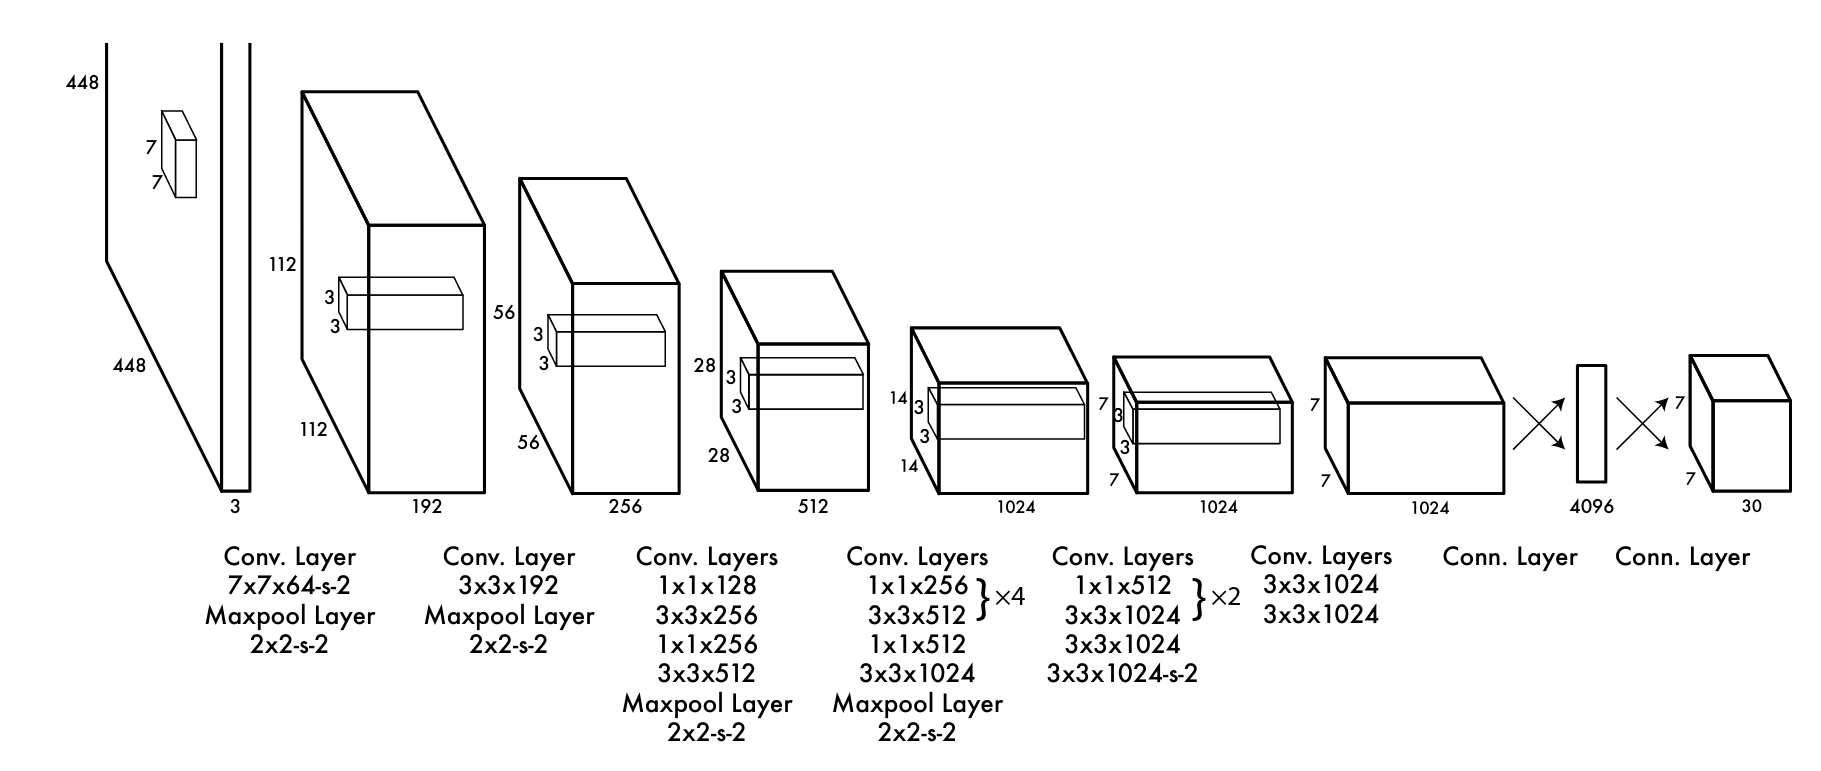
\includegraphics[width=\textwidth]{figures/paper/layers.png}
  \caption[The Architecture]{\textbf{The Architecture}. Our detection network has $24$ convolutional layers followed by $2$ fully connected layers. Alternating $1 \times 1$ convolutional layers reduce the features space from preceding layers. We pretrain the convolutional layers on the ImageNet classification task at half the resolution ($224 \times 224$ input image) and then double the resolution for detection.}
  \label{fig:figures/paper-iv/fig-3}
\end{figure}




\section{The Network}
The network structure looks like a normal CNN, with convolutional and max pooling layers, followed by 2 fully connected layers in the end:


\begin{table}[!h]
  \centering
  \caption[YOLO Network Structure]{YOLO Network Structure}
  \label{tab:yolo-network}
  {\renewcommand{\arraystretch}{1.3}
    \begin{tabular}{c c c}
      \toprule
      Name       &        Filters         & Output Dimension  \\
      \hline
      Conv 1     & 7 x 7 x 64, stride=2   & 224 x 224 x 64    \\
      Max Pool 1 & 2 x 2, stride=2        & 112 x 112 x 64    \\
      Conv 2     & 3 x 3 x 192            & 112 x 112 x 192   \\
      Max Pool 2 & 2 x 2, stride=2        & 56 x 56 x 192     \\
      Conv 3     & 1 x 1 x 128            & 56 x 56 x 128     \\
      Conv 4     & 3 x 3 x 256            & 56 x 56 x 256     \\
      Conv 5     & 1 x 1 x 256            & 56 x 56 x 256     \\
      Conv 6     & 1 x 1 x 512            & 56 x 56 x 512     \\
      Max Pool 3 & 2 x 2, stride=2        & 28 x 28 x 512     \\
      Conv 7     & 1 x 1 x 256            & 28 x 28 x 256     \\
      Conv 8     & 3 x 3 x 512            & 28 x 28 x 512     \\
      Conv 9     & 1 x 1 x 256            & 28 x 28 x 256     \\
      Conv 10    & 3 x 3 x 512            & 28 x 28 x 512     \\
      Conv 11    & 1 x 1 x 256            & 28 x 28 x 256     \\
      Conv 12    & 3 x 3 x 512            & 28 x 28 x 512     \\
      Conv 13    & 1 x 1 x 256            & 28 x 28 x 256     \\
      Conv 14    & 3 x 3 x 512            & 28 x 28 x 512     \\
      Conv 15    & 1 x 1 x 512            & 28 x 28 x 512     \\
      Conv 16    & 3 x 3 x 1024           & 28 x 28 x 1024    \\
      Max Pool 4 & 2 x 2, stride=2        & 14 x 14 x 1024    \\
      Conv 17    & 1 x 1 x 512            & 14 x 14 x 512     \\
      Conv 18    & 3 x 3 x 1024           & 14 x 14 x 1024    \\
      Conv 19    & 1 x 1 x 512            & 14 x 14 x 512     \\
      Conv 20    & 3 x 3 x 1024           & 14 x 14 x 1024    \\
      Conv 21    & 3 x 3 x 1024           & 14 x 14 x 1024    \\
      Conv 22    & 3 x 3 x 1024, stride=2 & 7 x 7 x 1024      \\
      Conv 23    & 3 x 3 x 1024           & 7 x 7 x 1024      \\
      Conv 24    & 3 x 3 x 1024           & 7 x 7 x 1024      \\
      FC 1       & -                      & 4096              \\
      FC 2       & -                      & 7 x 7 x 30 (1470) \\
\bottomrule
    \end{tabular}
  }
\end{table}

Note that the architecture was crafted for use in the Pascal VOC dataset, where the authors used $S=7$, $B=2$ and $C=20$. This explains why the final feature maps are $7 \times 7$, and also explains the size of the output $(7x7x(2 \times 5+20))$. Use of this network with a different grid size or different number of classes might require tuning of the layer dimensions. The authors mention that there is a fast version of YOLO, with fewer convolutional layers. The table~\ref{tab:yolo-network}, however, display the full version. The sequences of 1x1 reduction layers and 3x3 convolutional layers were inspired by the GoogLeNet (Inception) model. The final layer uses a linear activation function. All other layers use a leaky RELU $(\phi(x) = x, if x>0; 0.1x \ otherwise)$.

\section{The Loss Function}
The loss function start like this:
\begin{equation}
  \lambda_{coord} \sum_{i=0}^{S^2}\sum_{j=0}^B \mathbbm{1}_{ij}^{obj}[(x_i-\hat{x}_i)^2 + (y_i-\hat{y}_i)^2 ]
\label{yolo-loss-func}
\end{equation}


This equation computes the loss related to the predicted bounding box position $(x,y)$. Don’t worry about $\lambda$ for now, just consider it a given constant. The function computes a sum over each bounding box predictor $(j = 0..B)$ of each grid cell $(i = 0 .. S^2)$. $\mathbbm{1} obj$ is defined as follows:

\begin{itemize}
  \item 1, If an object is present in grid cell i and the jth bounding box predictor is “responsible” for that prediction
  \item 0, otherwise
\end{itemize}

But how do we know which predictor is responsible for the object? Quoting the original paper:
\begin{quote}
YOLO predicts multiple bounding boxes per grid cell. At training time we only want one bounding box predictor to be responsible for each object. We assign one predictor to be “responsible” for predicting an object based on which prediction has the highest current IOU with the ground truth.
\end{quote}

The other terms in the equation should be easy to understand: $(x, y)$ are the predicted bounding box position and $(\hat{x}, \hat{y})$ hat are the actual position from the training data.

Let’s move on to the second part:
\begin{equation}
  \lambda_{coord} \sum_{i=0}^{S^2}\sum_{j=0}^B \mathbbm{1}_{ij}^{obj}[(\sqrt{w_i}-\sqrt{\hat{w}_i})^2 +(\sqrt{h_i}-\sqrt{\hat{h}_i})^2 ]
\label{yolo-loss-func-2}
\end{equation}


This is the loss related to the predicted box width / height. The equation looks similar to the first one, except for the square root. Quoting the paper again:

\begin{quote}
Our error metric should reflect that small deviations in large boxes matter less than in small boxes. To partially address this we predict the square root of the bounding box width and height instead of the width and height directly.
  \end{quote}

    

Moving on to the third part:
\begin{equation}
  \sum_{i=0}^{S^2}\sum_{j=0}^B \mathbbm{1}_{ij}^{obj}(C_i - \hat{C}_i)^2 + \lambda_{noobj}\sum_{i=0}^{S^2}\sum_{j=0}^B \mathbbm{1}_{ij}^{noobj}(C_i - \hat{C}_i)^2
\label{yolo-loss-func-3}
\end{equation}


Here we compute the loss associated with the confidence score for each bounding box predictor. $C$ is the confidence score and $\hat{C}$ is the intersection over union of the predicted bounding box with the ground truth. $\mathbbm{1} obj$ is equal to one when there is an object in the cell, and 0 otherwise. $\mathbbm{1} noobj$  is the opposite.

The $\lambda $ parameters that appear here and also in the first part are used to differently weight parts of the loss functions. This is necessary to increase model stability. The highest penalty is for coordinate predictions $(\lambda coord = 5)$ and the lowest for confidence predictions when no object is present $(\lambda noobj = 0.5)$.

The last part of the loss function is the classification loss:
\begin{equation}
  \sum_{i=0}^{S^2} \mathbbm{1}_{i}^{obj}\sum_{c \in classes}(p_i(c) - \hat{p}_i(c))^2
\label{yolo-loss-func-4}
\end{equation}

It looks similar to a normal sum-squared error for classification, except for the $\mathbbm{1} obj$ term. This term is used because so we don’t penalize classification error when no object is present on the cell (hence the conditional class probability discussed earlier).

Note that the loss function only penalizes classification error if an object is present in that grid cell (hence the con-ditional class probability discussed earlier). It also only pe-nalizes bounding box coordinate error if that predictor is “responsible” for the ground truth box (i.e. has the highest IOU of any predictor in that grid cell). \cite{redmon2016look}


%=======================================================================
%%% References

% \clearpage
\phantomsection
\specialsection % put an indent, see preamble
\headerspecialsection

{\hypersetup{urlcolor=ntnu,linkcolor=sophia} % set clickable URL title color to black, not ntnu like in the main document

  \bibliographystyle{unsrtnat-mod}  % NATBIB ref style
  \bibliography{references}
}
